\documentclass[11pt,a4paper,oneside]{article}
\usepackage[latin1]{inputenc}
\usepackage{amsmath}
\usepackage{amsfonts}
\usepackage{amssymb}
\usepackage{graphicx}
\usepackage{color}
\usepackage {tikz}
\usetikzlibrary {er}
\usepackage[left=2.00cm, right=2.00cm, top=1.00cm]{geometry}
\graphicspath{{./}}

\begin{document}
	\title{DS 221 - Introduction to Scalable Systems \\ Assignment 1}
	\author{Shriram R. \\ M Tech (CDS) \\ 06-02-01-10-51-18-1-15763}
	\maketitle
	
	\section{Introduction}
	An efficient C program to multiply two square matrices has been developed by leveraging vectorization and locality of reference. The program has been tested for different matrix sizes and a comparison has been made with a naive implementation. The following sections will cover the program, analysis and performance results in detail.
	
	\section{Program (Optimized Version)}
	\begin{verbatim}
	#include <stdlib.h>
	#include <stdio.h>
	#include <time.h>
	
	double a[SIZE][SIZE], b[SIZE][SIZE], c[SIZE][SIZE]; // SIZE is set during compile
	
	int main()
	{
	    struct timespec start, end;
	    srand(time(NULL)); // Seed random number generator	    
	    for(int i=0; i<SIZE; i++) {
	        for(int j=0; j<SIZE; j++) {
	            a[i][j]=rand(); // Initialize with a random integer
	            b[i][j]=rand(); // Initialize with a random integer
	            c[i][j]=0;      // Initialize result matrix with 0
	        }
	    }	
	    clock_gettime(CLOCK_PROCESS_CPUTIME_ID, &start); // Capture start time	    
	    for(int i=0; i<SIZE; i++) {
	        for(int j=0; j<SIZE; j++) {
            for(int k=0; k<SIZE; k++) {
                c[i][k] += a[i][j]*b[j][k];
            }
        }
    }        
    clock_gettime(CLOCK_PROCESS_CPUTIME_ID, &end); // Capture end time        
    printf("%f s\n", (end.tv_nsec-start.tv_nsec)/1000000000.0+(end.tv_sec-start.tv_sec));
    return 0;
	}
	
	
	
	\end{verbatim}
	
    \section{Analysis}
    The idea behind the optimized version is that each row in the matrix C can be interpretated as a linear combination of the rows in matrix B using the values in rows of matrix A as weights. Precisely, \\
    \begin{center}
    	$R_C[i] = \sum_{j=1}^{n} A[i][j]*R_B[j]$ \\
    \end{center}
    where, $R_C[i]$ is the Row $i$ of matrix C and $R_B[j]$ is the Row $j$ of matrix B. This means that the elements of matrices are accessed in row major order thereby exploiting the spatial locality of reference. This improves the cache hit ratio substantially as compared to the naive version. \\ \\
    An important point to note is that the asymtotic time complexity of the optimized version is still $O(n^3)$ (same as the naive version). We have only decreased the constant multiplier.\\ \\
    Also, the 2D arrays have been declared as global variables in the program as these variables will have static allocation in the data segment. This is essential since the size of arrays could be huge and might not fit into the stack causing segmentation fault.\\ \\
    In addition to exploiting cache, vectorization of the for loop has been done by using relevant compiler flags. The innermost loop whick iterates on the columns of matrix B and C has been vectorized by the compiler.
    
    \section{Performance}
    The program has been tested in a personal computer having the following specification: Ubuntu 18.04 running on a Intel Core i5 8250U processor with L1, L2 and L3 cache size of 256KB, 1MB and 6MB respectively and 8GB of main memory. GCCv7.3.0 was used as the compiler. The time taken by the loop for different matrix sizes and programs is tabulated below along with a plot of time versus the matrix size, \\

    \begin{center}
	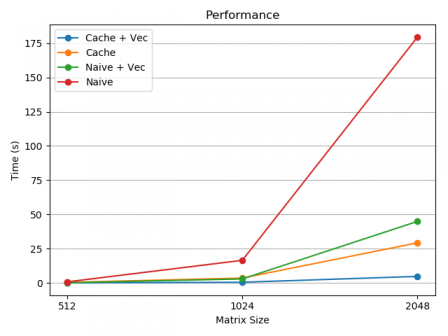
\includegraphics[scale=0.7]{mm_plot.png}
	\end{center}

    \begin{verbatim}
    
    
    \end{verbatim}

	\begin{center}
	\begin{tabular}{|l|l|l|l|}
		\hline
		Program & 512 & 1024 &  2048\\
		\hline
		Cache + Vec & 0.046s & 0.513s & 4.803s \\
		Cache & 0.447s & 3.595s & 29.292s \\
		Naive + Vec & 0.123s & 2.967s & 44.943s \\
		Naive & 0.798s & 16.532s & 179.477s \\				
		\hline
	\end{tabular}
	\end{center}

     \begin{verbatim}
    
    \end{verbatim}

    \section{Conclusion}
    It has been observed that the cache optimized and vectorized version of the program performs significantly better and scales well with the size of matrix. The optimized version took $0.513s$ to multiply 1024x1024 matrices of \emph{double} items. It is possible to improve the performance further by using divide and conquer algorithm like Strassen's which has a better complexity than $O(n^3)$. 
    
    \section{References}
    
    \begin{list}{*}{}
    	\item https://gcc.gnu.org/projects/tree-ssa/vectorization.html
    	\item https://stackoverflow.com/questions/1847789/segmentation-fault-on-large-array-sizes
    	\item https://linux.die.net/man/3/clock\_gettime
    	\item DS 221 Course lecture notes
    \end{list}

\end{document}